\subsubsection{19.12.2015 (Competition)}
\textit{\textbf{Time frame:}} 10:00-22:00

Today was the first day of competition "Robofest-Ryazan ". Today there were only training matches and time for preparing robots. Our team provided the organisers of this competition with original FTC 2016 playing field. The field was assembled and trainings started.

We tested the elevator, but it was found that the toothing between gears on the winch is not sufficient, so they are slipping. It made impossible to extract the slats because motors couldn't provide the coils with enough power. Due to this, we could only deliver debris to the floor goal during the match.

\begin{figure}[H]
	\begin{minipage}[h]{0.47\linewidth}
		\center{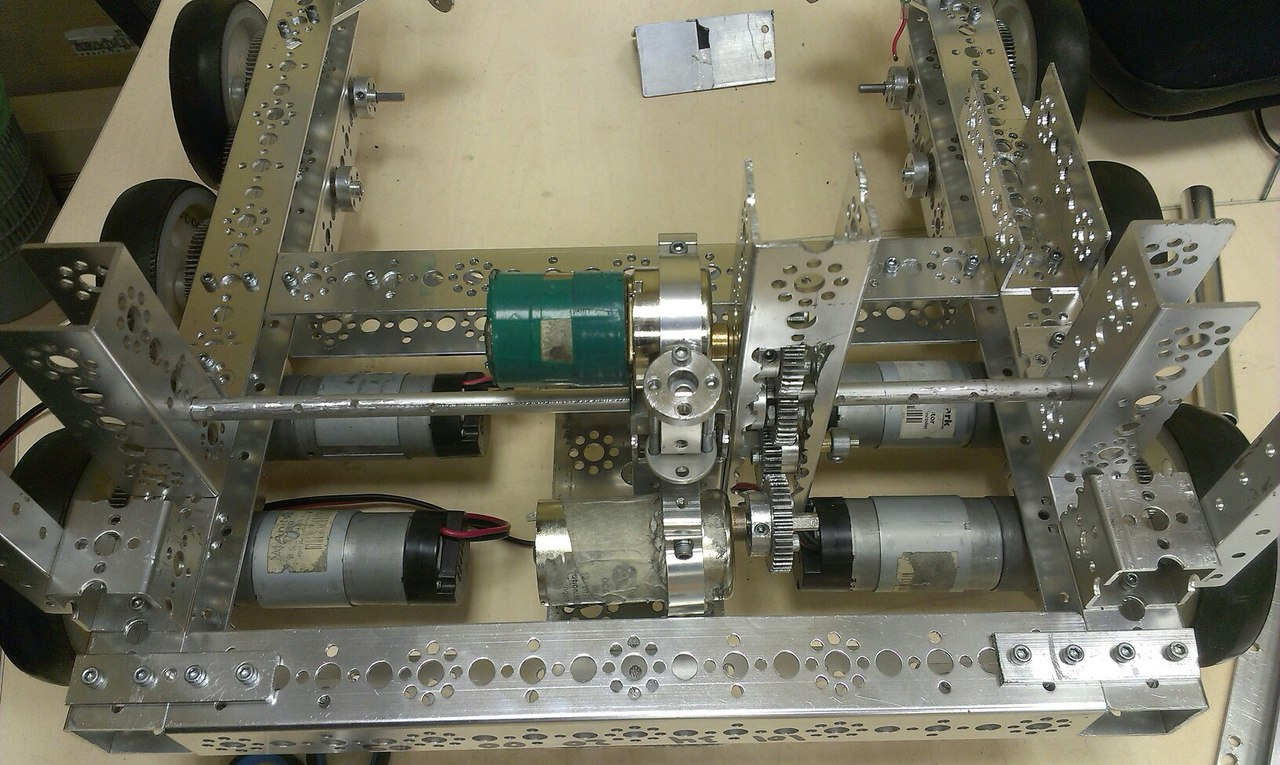
\includegraphics[scale=0.4]{3Engineering/5Team_meetings/days_of_meetings/2015.12.19/images/01}}
		\caption{Testing elevator on the field}
	\end{minipage}
	\hfill
	\begin{minipage}[h]{0.47\linewidth}
		\center{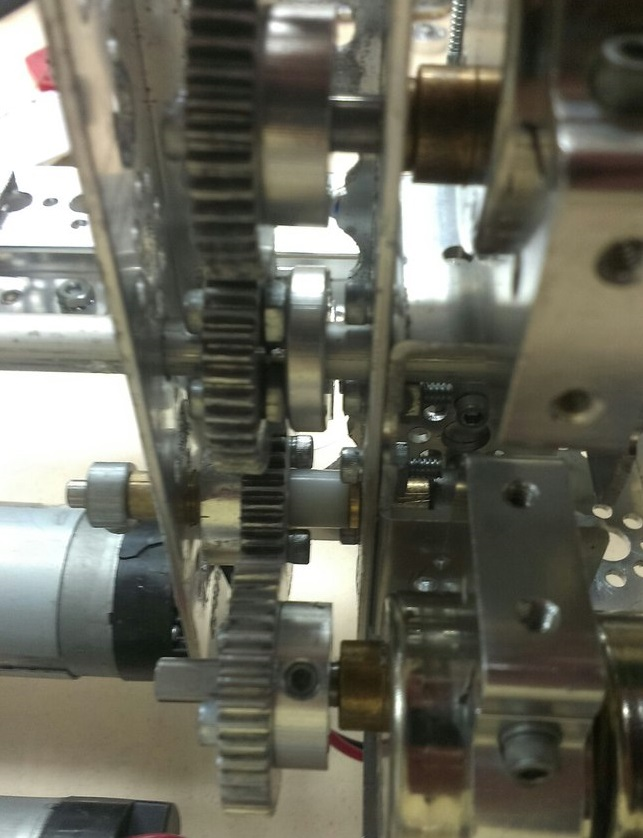
\includegraphics[scale=0.4]{3Engineering/5Team_meetings/days_of_meetings/2015.12.19/images/02}}
		\caption{Programming and technical inspection}
	\end{minipage}
\end{figure}